\begin{priprava}{5}{}{Ploščina trikotnika}{Pravokotni koordinatni sistem}{frontalna}{drsnice, projekcija, tabla}


    
    \section{Ploščina trikotnika}

        \begin{wrapfigure}{r}{0.38\textwidth}
            \vskip-2em
        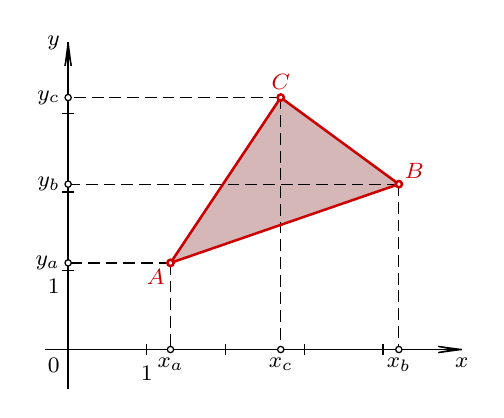
\begin{tikzpicture}
            % \clip (0,0) rectangle (14.000000,10.000000);
            {\footnotesize
            
            % Drawing 2D Cartesian system
            \draw (2.000000,2.000000) node [anchor=north east] { $0$ };%
            \draw [line width=0.016cm] (2.000000,1.925000) -- (2.000000,2.075000);%
            \draw (3.000000,1.900000) node [anchor=north] { $1$ };%
            \draw [line width=0.016cm] (3.000000,1.925000) -- (3.000000,2.075000);%
            % \draw (4.000000,2.000000) node [anchor=north] { $2$ };%
            \draw [line width=0.016cm] (4.000000,1.925000) -- (4.000000,2.075000);%
            % \draw (5.000000,2.000000) node [anchor=north] { $3$ };%
            \draw [line width=0.016cm] (5.000000,1.925000) -- (5.000000,2.075000);%
            % \draw (6.000000,2.000000) node [anchor=north] { $4$ };%
            \draw [line width=0.016cm] (6.000000,1.925000) -- (6.000000,2.075000);%
            % \draw (7.000000,2.000000) node [anchor=north] { $5$ };%
            % \draw [line width=0.016cm] (7.000000,1.925000) -- (7.000000,2.075000);%
            \draw (2.000000,2.800000) node [anchor=east] { $1$ };%
            \draw [line width=0.016cm] (1.925000,3.000000) -- (2.075000,3.000000);%
            % \draw (2.000000,4.000000) node [anchor=east] { $2$ };%
            \draw [line width=0.016cm] (1.925000,4.000000) -- (2.075000,4.000000);%
            % \draw (2.000000,5.000000) node [anchor=east] { $3$ };%
            \draw [line width=0.016cm] (1.925000,5.000000) -- (2.075000,5.000000);%
            \draw (7.000000,2.000000) node [anchor=north] { $x$ };%
            \draw (2.000000,5.900000) node [anchor=east] { $y$ };%
            \draw [line width=0.016cm] (1.700000,2.000000) -- (3.260000,2.000000);%
            \draw [line width=0.016cm] (3.340000,2.000000) -- (4.660000,2.000000);%
            \draw [line width=0.016cm] (4.740000,2.000000) -- (6.160000,2.000000);%
            \draw [line width=0.016cm] (6.240000,2.000000) -- (7.000000,2.000000);%
            \draw [line width=0.016cm] (6.702567,2.039158) -- (7.000000,2.000000);%
            \draw [line width=0.016cm] (6.702567,2.039158) -- (6.900000,2.000000);%
            \draw [line width=0.016cm] (6.702567,1.960842) -- (7.000000,2.000000);%
            \draw [line width=0.016cm] (6.702567,1.960842) -- (6.900000,2.000000);%
            \draw [line width=0.016cm] (2.000000,1.500000) -- (2.000000,3.060000);%
            \draw [line width=0.016cm] (2.000000,3.140000) -- (2.000000,4.060000);%
            \draw [line width=0.016cm] (2.000000,4.140000) -- (2.000000,5.160000);%
            \draw [line width=0.016cm] (2.000000,5.240000) -- (2.000000,5.900000);%
            \draw [line width=0.016cm] (1.960842,5.602567) -- (2.000000,5.900000);%
            \draw [line width=0.016cm] (1.960842,5.602567) -- (2.000000,5.800000);%
            \draw [line width=0.016cm] (2.039158,5.602567) -- (2.000000,5.900000);%
            \draw [line width=0.016cm] (2.039158,5.602567) -- (2.000000,5.800000);%
            
            % Changing color 213 183 183
            \definecolor{r213g183b183}{rgb}{0.835294,0.717647,0.717647}%
            \color{r213g183b183}% 
            
            % Filling triangle A B C
            \fill (3.300000,3.100000) -- (6.200000,4.100000) -- (4.700000,5.200000);%
            
            % Changing color 0 0 0
            \definecolor{r0g0b0}{rgb}{0.000000,0.000000,0.000000}%
            \color{r0g0b0}% 
            
            % Drawing segment A x_a
            \draw [line width=0.016cm] (3.300000,3.060000) -- (3.300000,2.950000);%
            \draw [line width=0.016cm] (3.300000,2.875000) -- (3.300000,2.725000);%
            \draw [line width=0.016cm] (3.300000,2.650000) -- (3.300000,2.500000);%
            \draw [line width=0.016cm] (3.300000,2.425000) -- (3.300000,2.275000);%
            \draw [line width=0.016cm] (3.300000,2.200000) -- (3.300000,2.050000);%
            
            % Drawing segment A y_a
            \draw [line width=0.016cm] (3.260000,3.100000) -- (3.150000,3.100000);%
            \draw [line width=0.016cm] (3.075000,3.100000) -- (2.925000,3.100000);%
            \draw [line width=0.016cm] (2.850000,3.100000) -- (2.700000,3.100000);%
            \draw [line width=0.016cm] (2.625000,3.100000) -- (2.475000,3.100000);%
            \draw [line width=0.016cm] (2.400000,3.100000) -- (2.250000,3.100000);%
            \draw [line width=0.016cm] (2.175000,3.100000) -- (2.040000,3.100000);%
            
            % Drawing segment B x_b
            \draw [line width=0.016cm] (6.200000,4.060000) -- (6.200000,3.950000);%
            \draw [line width=0.016cm] (6.200000,3.875000) -- (6.200000,3.725000);%
            \draw [line width=0.016cm] (6.200000,3.650000) -- (6.200000,3.500000);%
            \draw [line width=0.016cm] (6.200000,3.425000) -- (6.200000,3.275000);%
            \draw [line width=0.016cm] (6.200000,3.200000) -- (6.200000,3.050000);%
            \draw [line width=0.016cm] (6.200000,2.975000) -- (6.200000,2.825000);%
            \draw [line width=0.016cm] (6.200000,2.750000) -- (6.200000,2.600000);%
            \draw [line width=0.016cm] (6.200000,2.525000) -- (6.200000,2.375000);%
            \draw [line width=0.016cm] (6.200000,2.300000) -- (6.200000,2.150000);%
            \draw [line width=0.016cm] (6.200000,2.075000) -- (6.200000,2.040000);%
            
            % Drawing segment B y_b
            \draw [line width=0.016cm] (6.160000,4.100000) -- (6.050000,4.100000);%
            \draw [line width=0.016cm] (5.975000,4.100000) -- (5.825000,4.100000);%
            \draw [line width=0.016cm] (5.750000,4.100000) -- (5.600000,4.100000);%
            \draw [line width=0.016cm] (5.525000,4.100000) -- (5.375000,4.100000);%
            \draw [line width=0.016cm] (5.300000,4.100000) -- (5.150000,4.100000);%
            \draw [line width=0.016cm] (5.075000,4.100000) -- (4.925000,4.100000);%
            \draw [line width=0.016cm] (4.850000,4.100000) -- (4.700000,4.100000);%
            \draw [line width=0.016cm] (4.625000,4.100000) -- (4.475000,4.100000);%
            \draw [line width=0.016cm] (4.400000,4.100000) -- (4.250000,4.100000);%
            \draw [line width=0.016cm] (4.175000,4.100000) -- (4.025000,4.100000);%
            \draw [line width=0.016cm] (3.950000,4.100000) -- (3.800000,4.100000);%
            \draw [line width=0.016cm] (3.725000,4.100000) -- (3.575000,4.100000);%
            \draw [line width=0.016cm] (3.500000,4.100000) -- (3.350000,4.100000);%
            \draw [line width=0.016cm] (3.275000,4.100000) -- (3.125000,4.100000);%
            \draw [line width=0.016cm] (3.050000,4.100000) -- (2.900000,4.100000);%
            \draw [line width=0.016cm] (2.825000,4.100000) -- (2.675000,4.100000);%
            \draw [line width=0.016cm] (2.600000,4.100000) -- (2.450000,4.100000);%
            \draw [line width=0.016cm] (2.375000,4.100000) -- (2.225000,4.100000);%
            \draw [line width=0.016cm] (2.150000,4.100000) -- (2.040000,4.100000);%
            
            % Drawing segment C x_c
            \draw [line width=0.016cm] (4.700000,5.160000) -- (4.700000,5.050000);%
            \draw [line width=0.016cm] (4.700000,4.975000) -- (4.700000,4.825000);%
            \draw [line width=0.016cm] (4.700000,4.750000) -- (4.700000,4.600000);%
            \draw [line width=0.016cm] (4.700000,4.525000) -- (4.700000,4.375000);%
            \draw [line width=0.016cm] (4.700000,4.300000) -- (4.700000,4.150000);%
            \draw [line width=0.016cm] (4.700000,4.075000) -- (4.700000,3.925000);%
            \draw [line width=0.016cm] (4.700000,3.850000) -- (4.700000,3.700000);%
            \draw [line width=0.016cm] (4.700000,3.625000) -- (4.700000,3.475000);%
            \draw [line width=0.016cm] (4.700000,3.400000) -- (4.700000,3.250000);%
            \draw [line width=0.016cm] (4.700000,3.175000) -- (4.700000,3.025000);%
            \draw [line width=0.016cm] (4.700000,2.950000) -- (4.700000,2.800000);%
            \draw [line width=0.016cm] (4.700000,2.725000) -- (4.700000,2.575000);%
            \draw [line width=0.016cm] (4.700000,2.500000) -- (4.700000,2.350000);%
            \draw [line width=0.016cm] (4.700000,2.275000) -- (4.700000,2.125000);%
            \draw [line width=0.016cm] (4.700000,2.050000) -- (4.700000,2.040000);%
            
            % Drawing segment C y_c
            \draw [line width=0.016cm] (4.660000,5.200000) -- (4.550000,5.200000);%
            \draw [line width=0.016cm] (4.475000,5.200000) -- (4.325000,5.200000);%
            \draw [line width=0.016cm] (4.250000,5.200000) -- (4.100000,5.200000);%
            \draw [line width=0.016cm] (4.025000,5.200000) -- (3.875000,5.200000);%
            \draw [line width=0.016cm] (3.800000,5.200000) -- (3.650000,5.200000);%
            \draw [line width=0.016cm] (3.575000,5.200000) -- (3.425000,5.200000);%
            \draw [line width=0.016cm] (3.350000,5.200000) -- (3.200000,5.200000);%
            \draw [line width=0.016cm] (3.125000,5.200000) -- (2.975000,5.200000);%
            \draw [line width=0.016cm] (2.900000,5.200000) -- (2.750000,5.200000);%
            \draw [line width=0.016cm] (2.675000,5.200000) -- (2.525000,5.200000);%
            \draw [line width=0.016cm] (2.450000,5.200000) -- (2.300000,5.200000);%
            \draw [line width=0.016cm] (2.225000,5.200000) -- (2.075000,5.200000);%
            
            % Marking point x_a by circle
            \draw [line width=0.016cm] (3.300000,2.000000) circle (0.040000);%
            \draw (3.300000,2.000000) node [anchor=north] { $x_a$ };%
            
            % Marking point x_b by circle
            \draw [line width=0.016cm] (6.200000,2.000000) circle (0.040000);%
            \draw (6.200000,2.000000) node [anchor=north] { $x_b$ };%
            
            % Marking point y_a by circle
            \draw [line width=0.016cm] (2.000000,3.100000) circle (0.040000);%
            \draw (2.000000,3.100000) node [anchor=east] { $y_a$ };%
            
            % Marking point y_b by circle
            \draw [line width=0.016cm] (2.000000,4.100000) circle (0.040000);%
            \draw (2.000000,4.100000) node [anchor=east] { $y_b$ };%
            
            % Marking point x_c by circle
            \draw [line width=0.016cm] (4.700000,2.000000) circle (0.040000);%
            \draw (4.700000,2.000000) node [anchor=north] { $x_c$ };%
            
            % Marking point y_c by circle
            \draw [line width=0.016cm] (2.000000,5.200000) circle (0.040000);%
            \draw (2.000000,5.200000) node [anchor=east] { $y_c$ };%
            
            % Changing color 204 0 0
            \definecolor{r204g0b0}{rgb}{0.800000,0.000000,0.000000}%
            \color{r204g0b0}% 
            
            % Drawing segment A B
            \draw [line width=0.032cm] (3.337815,3.113040) -- (6.162185,4.086960);%
            
            % Drawing segment C B
            \draw [line width=0.032cm] (4.732256,5.176345) -- (6.167744,4.123655);%
            
            % Drawing segment A C
            \draw [line width=0.032cm] (3.322188,3.133282) -- (4.677812,5.166718);%
            
            % Marking point A by circle
            \draw [line width=0.032cm] (3.300000,3.100000) circle (0.040000);%
            \draw (3.330000,3.130000) node [anchor=north east] { $A$ };%
            
            % Marking point B by circle
            \draw [line width=0.032cm] (6.200000,4.100000) circle (0.040000);%
            \draw (6.170000,4.070000) node [anchor=south west] { $B$ };%
            
            % Marking point C by circle
            \draw [line width=0.032cm] (4.700000,5.200000) circle (0.040000);%
            \draw (4.700000,5.200000) node [anchor=south] { $C$ };%
            \color{black}
            }
            \end{tikzpicture}
        \end{wrapfigure}

        Ploščina trikotnika $\triangle ABC$ z oglišči $A(x_a,y_a)$, $B(x_b,y_b)$ in $C(x_c,y_c)$ je
        $$ \begin{aligned} S &= \frac{1}{2}\cdot orient \cdot \begin{vmatrix} x_b-x_a & y_b-y_a \\ x_c-x_a & y_c-y_a \end{vmatrix} 
                \\ &= \frac{orient}{2}  \left[(x_b-x_a)(y_c-y_a)-(y_b-y_a)(x_c-x_a)\right], \end{aligned} $$
        kjer je $orient=\begin{cases} 1; & \triangle ABC ~pozitivno~orientiran \\ -1; & \triangle ABC ~negativno~orientiran \end{cases}. $






    % naloge

    ~\\~\\~\\

        \begin{naloga}
            Narišite trikotnik $\triangle ABC$ in izračunajte njegovo ploščino.
            \begin{itemize}
                \item $A(-4,-2)$, $B(5,1)$ in $C(-2,5)$ 
                \item $A(2,1)$, $B(-5,1)$ in $C(2,6)$ 
            \end{itemize}
        \end{naloga}

        \begin{naloga}
            Ali so točke kolinearne?
            \begin{itemize}
                \item $P(-4,-5)$, $Q(4,-1)$ in $R(10,2)$ 
                \item $X(1,-7)$, $Y(-2,2)$ in $Z(3,2)$ 
            \end{itemize}
        \end{naloga}

        \begin{naloga}
            Določite $x$ tako, da bo trikotnik $\triangle ABC$, z oglišči v $A(-2,-3)$, $B(5,3)$ in $C(x,-1)$, negativno orientiran 
            in bo imel ploščino $17$. 
        \end{naloga}
       
        \begin{naloga}
            Določite $p$ tako, da bo imel trikotnik $\triangle ABC$, z oglišči v $A(2,3)$, $B(p,-3)$ in $C(-1,6)$, ploščino $18$. 
        \end{naloga}

        \begin{naloga}
            Dani sta točki $A(2,-4)$ in $B(8,3)$. Določite koordinati točke $C$, ki leži na simetrali lihih kvadrantov, 
            da bo trikotnik $\triangle ABC$ pozitivno orientiran in bo imel ploščino $17$.
        \end{naloga}




\end{priprava}